\chapter{Conceitos básicos}\label{cap_conceitos}

O foco deste capítulo é introduzir os tópicos mais relevantes para o trabalho, de forma que o leitor consiga
entender o conteúdo independente de conhecimento prévio.
Neste capítulo serão abordados os tópicos relacionados a ANN (\autoref{cap_conceitos_ann}),
CNN (\autoref{cap_conceitos_cnn}), \textit{Data augmentation} (\autoref{cap_conceitos_data_augmentation}),
transferência de conhecimento (\autoref{cap_conceitos_transferencia}), técnicas de compressão para redes neurais
(\autoref{cap_conceitos_compressao_redes}) e otimização Bayesiana (\autoref{cap_conceitos_bayesiana}).

\section{Redes Neurais Artificiais}\label{cap_conceitos_ann}
Redes Neurais Artificiais é composta por neurônios interconectados, onde cada um é responsável por fazer um
processamento simples.
% são neurônios interconectados que realizam um processamento simples.
Dentro dessa estrutura cada neurônio reforça ou enfraquece a conexão com um dos neurônios da camada anterior, assim
replicando o processo de aprendizagem do cérebro humano \cite{ml-faceli}.
A \autoref{cap_conceitos_ann_exemplo_ann} ilustra uma ANN simples.

\begin{figure}[htb]
	\caption {\label{cap_conceitos_ann_exemplo_ann}Exemplo de uma ANN}
	\begin{center}
		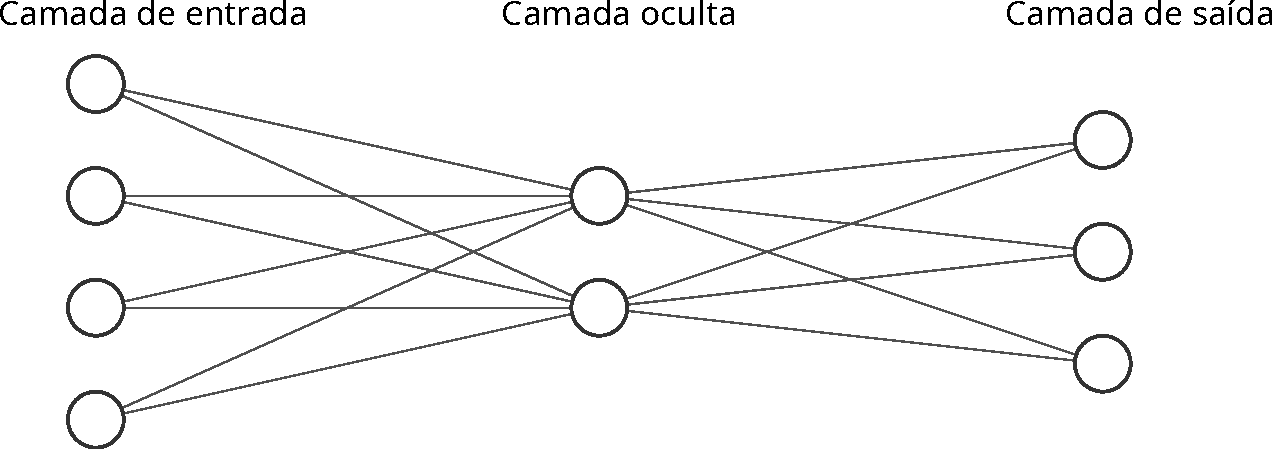
\includegraphics[scale=0.5]{Imagens/exemplo_nn}
	\end{center}
	\legend {Fonte: Autor}
\end{figure}

O neurônio é uma parte fundamental de uma ANN, nele que o aprendizado é armazenado através do reforço de conexões com
outros neurônios. Esse reforço é o peso da conexão, ele é multiplicado pela entrada e somado com os outros valores,
como é demonstrado na equação \ref{eq_neuronio}, onde $x$ é um vetor com os valores de entrada do neurônio, $w$
é um vetor com os pesos de cada entrada e $b$ é o viés (\textit{bias}) do modelo.
Depois disso, os valores passam por uma função de ativação $g(x)$ (\ref
{eq_ativacao}), que é responsável por transformar estes dados antes que sejam passados para a próxima etapa, por esta
razão, a função de ativação também é chamada função de transferência.

\begin{equation}\label{eq_neuronio}
u = \sum x_i w_i
\end{equation}
\begin{equation}\label{eq_ativacao}
y = g(u + b)
\end{equation}

\begin{figure}[htb]
	\caption {\label{cap_conceitos_ex_neuronio} Exemplo de um neurônio artificial}
	\begin{center}
		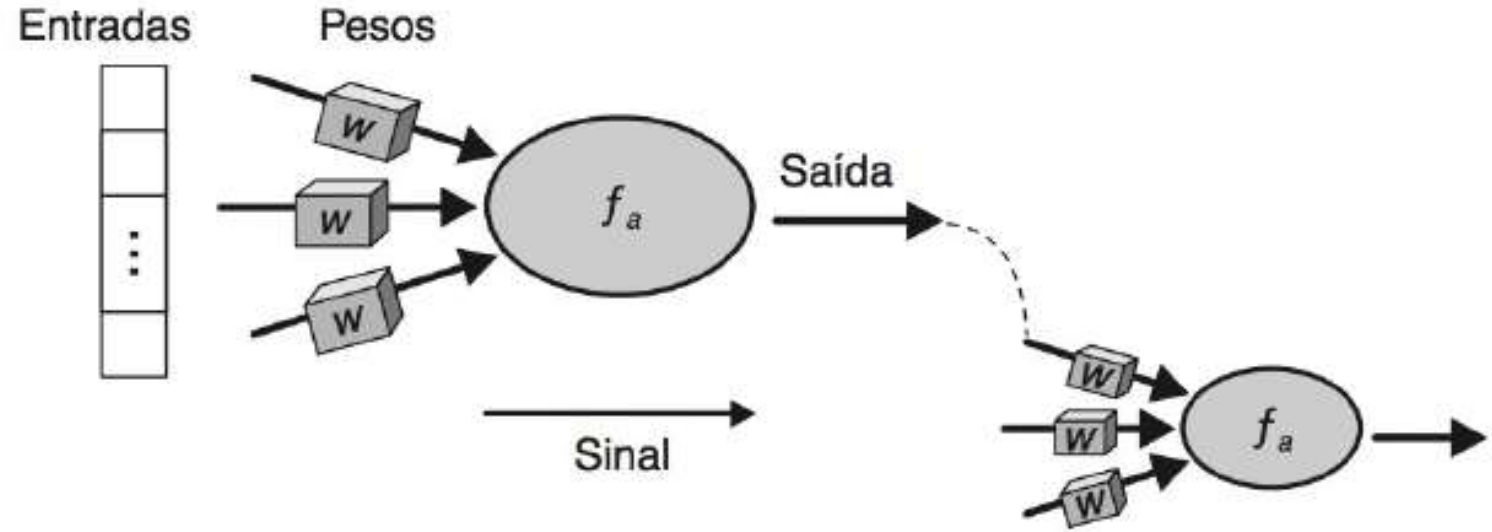
\includegraphics[scale=0.3]{Imagens/exemplo_neuronio_artificial}
	\end{center}
	\legend{Fonte: \cite{ml-faceli}}
\end{figure}

\section{Redes Neurais Convolucionais}\label{cap_conceitos_cnn}
Redes Neurais Convolucionais são Redes Neurais Artificiais que utilizam a operação de convolução para o processamento e
análise de dados no formato de \textit{grid} (grade).
Por exemplo, uma imagem, que pode ser representada no formato 2-D \cite{Goodfellow-et-al-2016}.

% TODO: Adicionar ponto e vírgula
A arquitetura de uma CNN tem como componentes principais as camadas convolucionais (\autoref{cap_conceitos_cnn_conv}),
que tem como o objetivo extrair as características dos dados de entrada;
\textit{pooling} (\autoref{cap_conceitos_cnn_pooling}), que realça certos pontos da sua entrada, reduzindo o tamanho
final da sua saída;
a camada totalmente conectada (\autoref{cap_conceitos_cnn_totalmente}), que aprende a interpretar esses dados,
para que a rede consiga realizar o processo de classificação.
Na \autoref{exemplo_lenet} é mostrada a ilustração da arquitetura de uma CNN.

\begin{figure}[htb]
	\caption {\label{exemplo_lenet} Arquitetura da LeNet}
	\begin{center}
		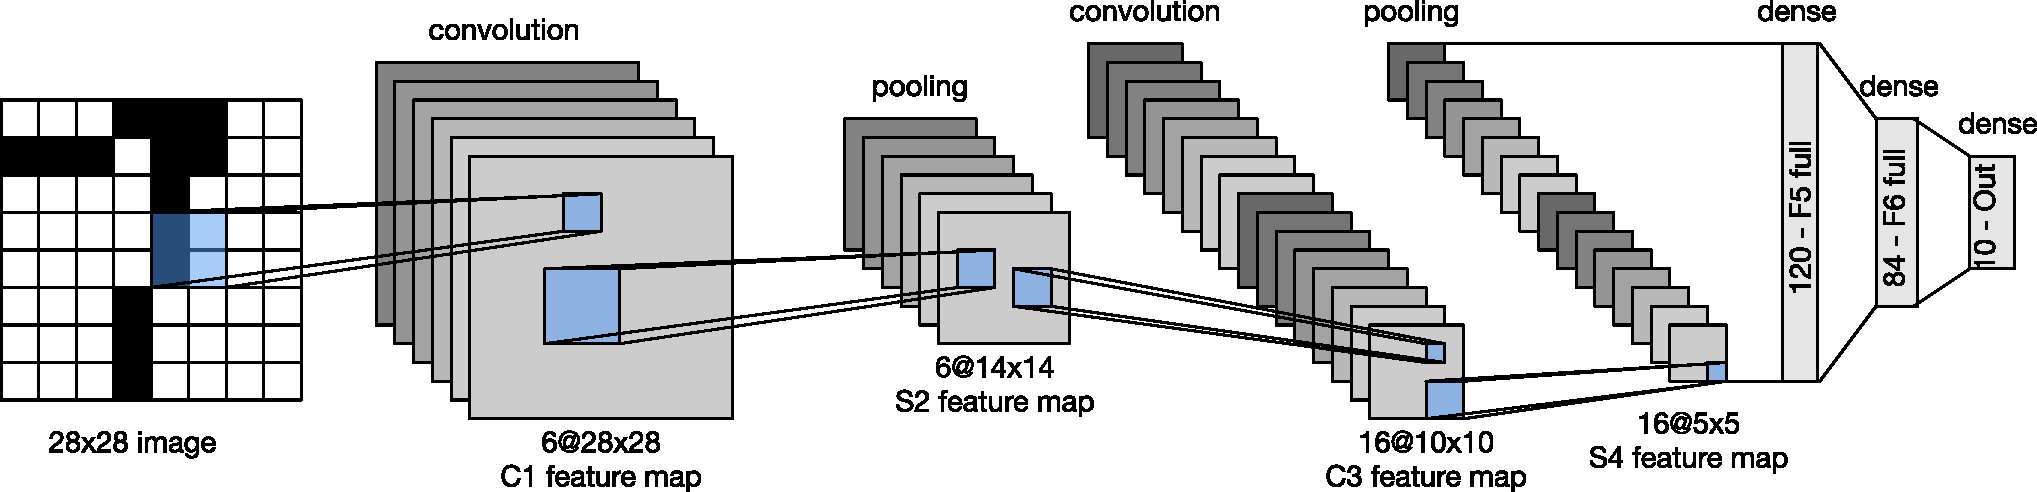
\includegraphics[scale=0.5]{Imagens/lenet}
	\end{center}
	\legend{Fonte: \citeonline{zhang2023dive}}
\end{figure}

\subsection{Camada de Convolução}\label{cap_conceitos_cnn_conv}
Nessa camada são aplicados filtros (matriz de pesos) nos dados de entrada, onde esses filtros deslizam ao longo da
grade de entrada executando operações de multiplicação e soma em cada elemento da matriz de entrada, com o objetivo de
gerar um mapa de características (\textit{feature map}).
O objetivo desses filtros é realçar as características dos dados de entrada. Alguns padrões como curvas e linhas podem ser
reconhecidos por estas operações de filtragem.
A \autoref{exemplo_conv}, é um exemplo da operação de convolução sendo aplicada em uma matriz.

\begin{figure}[htb]
	\caption {\label{exemplo_conv} Exemplo de convolução}
	\begin{center}
		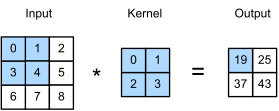
\includegraphics[scale=1.0]{Imagens/conv}
	\end{center}
	\legend{Fonte: \citeonline{zhang2023dive}}
\end{figure}

\subsection{Camada de \textit{pooling}}\label{cap_conceitos_cnn_pooling}
% ---
A abordagem da camada de \textit{pooling} é relativamente parecida com a camada de convolução,
uma matriz desliza pelas células da imagem, salvando apenas um dos valores dessa área na matriz de saída.
Esta operação reduz o tamanho da matriz de entrada, fazendo com que o poder computacional necessário seja reduzido,
junto com o uso de memória.

Existem diversos tipos de \textit{pooling}, min, \textit{average} e max, onde cada um foca em extrair um valor dos
dados de entrada na matriz. O tipo mais comum de \textit{pooling} é o max, que salva apenas o maior valor da área,
além de reduzir o tamanho da matriz de entrada ele consegue realçar algumas características mais expressivas da matriz.
A \autoref{exemplo_pooling} demonstra uma operação de max \textit{pooling} em uma matriz.

\begin{figure}[htb]
	\caption {\label{exemplo_pooling} Exemplo de max \textit{pooling}}
	\begin{center}
		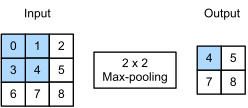
\includegraphics[scale=1.0]{Imagens/maxpooling}
	\end{center}
	\legend{Fonte: \citeonline{zhang2023dive}}
\end{figure}

\subsection{Camada totalmente conectada}\label{cap_conceitos_cnn_totalmente}
% ---
A camada totalmente conectada (\textit{fully connected layer}) é uma das últimas camadas de uma CNN.
Depois das camadas anteriores extraírem as características da imagem, ela é responsável por
aprender a interpretar essas características e inferir um resultado a partir do seu treinamento.
Essa camada é uma ANN (\autoref{cap_conceitos_ann}) que geralmente é focada em realizar a classificação dos dados
de entrada.

\section{\textit{Data augmentation}}\label{cap_conceitos_data_augmentation}
% ---
CNN tem um bom desempenho em tarefas de visão computacional. Entretanto, esse tipo de rede neural precisa de uma
grande quantidade de dados no treinamento para não sofrer de superajuste (\textit{overfitting})
\cite{shorten2019survey}.
O objetivo do \textit{data augmentation} (aumento de dados) é gerar mais dados a partir de um conjunto de dados
que já existe, aplicando algumas transformações geométricas ou espaciais, ou realizando injeção de ruído nas imagens
originais.

Na \autoref{cap_conceitos_exemplo_da}, é apresentado um exemplo de uma imagem que sofreu uma transformação para efetuar
um \textit{data augmentation}.
Nesse caso, uma que foi revertida (\textit{flip}), gerando um novo dado para o \text{dataset}

\begin{figure}[htb]
	\caption {\label{cap_conceitos_exemplo_da}Exemplo de uma transformação utilizando \textit{data augmentation}}
	\begin{center}
		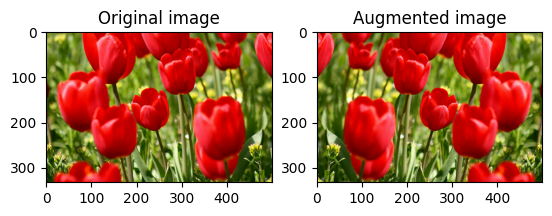
\includegraphics[scale=1]{Imagens/exemplo_da}
	\end{center}
	\legend {Fonte: \citeonline{tf2guia}}
\end{figure}

% TODO: Continuar
\section{Transferência de conhecimento}\label{cap_conceitos_transferencia}
% ---
Transferência de conhecimento consiste em usar um modelo pré-treinado em uma base de dados específica e aproveitar
o conhecimento adquirido durante esse treinamento para um novo conjunto de dados.
% TODO: Ver como explicar melhor
% É necessário que o problema do \textit{dataset} (conjunto de dados) atual seja um subconjunto do problema
% que foi usado para treinar o modelo base.
% Por exemplo, um modelo Professor que reconhece animais e um Aluno que reconhece gatos e cachorros.

Para realizar a transferência de conhecimento é necessário adaptar a camada de entrada e de saída
(totalmente conectada) do modelo base, para que ocorra um pré-processamento dos dados de entrada
(antes deles serem passados para o modelo base), além disso é necessário definir e treinar a camada totalmente
conectada com o \textit{dataset} do problema.

\section{Métodos de compressão para Redes Neurais}\label{cap_conceitos_compressao_redes}
ANN são utilizadas em várias aplicações, demonstrando habilidades no campo de visão computacional.
No entanto, redes com arquiteturas complexas são um desafio para a implantação em tempo real e necessitam de uma
grande quantidade de energia e poder computacional \cite{LIANG2021370}.
Por causa disso foram desenvolvidos métodos para reduzir o tamanho dessas redes, as tornando mais eficientes.
Nesse trabalho os métodos de poda (\autoref{poda}), quantização (\autoref{quantizacao}) e destilação do conhecimento
(\autoref{conceitos_destilacao}) serão usados.

\subsection{\textit{Pruning}(Poda)}\label{poda}

A poda de redes neurais tem como foco eliminar conexões ou neurônios que não apresentam uma grade contribuição para a
rede.
Essa operação, é muito vantajosa para diminuir a pegada de memória (\textit{memory footprint}) da rede, pois ela reduz
a quantidade de parâmetros redundantes ou que não contribuem muito para a precisão dos resultados.

A operação de poda procura pesos com valores abaixo de um determinado limiar e os muda para a zero, assim deixando
a rede neural mais esparsa, o que facilita o processo de compressão.
O processo de poda pode reduzir o \textit{overfitting} da rede, uma vez que remove pesos pouco importantes ou redundantes
da rede.
Esse processo geralmente é divido em dois, poda estática (\textit{static pruning}), que tem todas as etapas de poda
executadas off-line (antes da inferência), e poda dinâmica (\textit{dynamic pruning}), que é realizada junto com
o processo de execução do modelo, permitindo que os nós relevantes sejam identificados. A
\autoref{cap_conceitos_tipos_poda} ilustra o fluxo dos dois tipos de poda.

\begin{figure}[htb]
	\caption {\label{cap_conceitos_tipos_poda}Fluxo dos tipos de poda}
	\begin{center}
		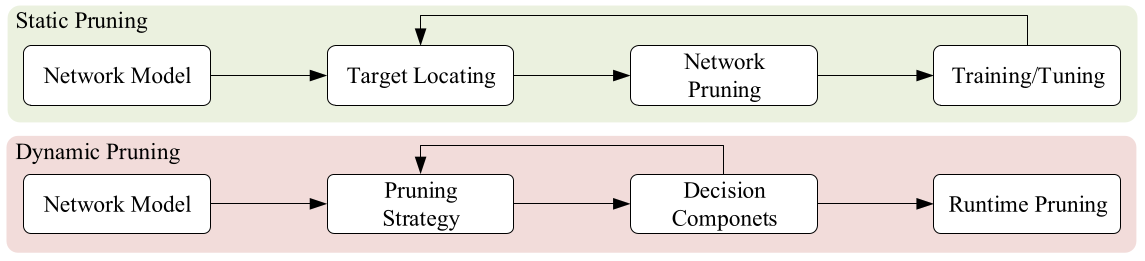
\includegraphics[scale=0.5]{Imagens/categorias-poda}
	\end{center}
	\legend {Fonte: \cite{LIANG2021370}}
\end{figure}

\subsection{Quantização}\label{quantizacao}

Quantização reduz a computação diminuindo a precisão dos tipos de dados. Pesos, \textit{bias} (vieses) e ativações
geralmente devem ser quantizadas para inteiros de 8 bits, embora implementações menores que 8 bits sejam discutidas
incluindo redes neurais binárias. \cite{LIANG2021370}

\subsection{Destilação de conhecimento (Professor-Aluno)}\label{conceitos_destilacao}

Destilação de conhecimento ou \textit{knowledge distillation} \cite{hinton2015distilling}, é uma técnica que tem
como objetivo treinar um modelo Aluno (menor e sem pré-treinamento) com um modelo Professor
(maior e com pré-treinamento). Ela é amplamente utilizada para as áreas de visão computacional e linguagem natural,
e tem como objetivo reduzir o tamanho do modelo final (Aluno).

Para transferir o conhecimento do modelo Professor para o Aluno, a técnica utiliza os \textit{logits} (entrada da
função de ativação final \textit{softmax}) no lugar da classe prevista. Além disso, são utilizado os
\textit{soft targets} (probabilidades das classes previstas pelo modelo Professor) junto com os
\textit{hard targets} (classe esperada).

% NOTE: Talvez detalhar a temperatura?

\section{Otimização Bayesiana}\label{cap_conceitos_bayesiana}
% ---
A otimização Bayesiana é um método utilizado para a otimização de hiperparâmetros em modelos de aprendizagem de
máquina, especialmente do tipo caixa preta (\textit{black box}), como CNN.
Esse método de otimização possui dois componentes principais, o modelo estatístico Bayesiano, que serve para modelar a
função alvo, e a função de aquisição, que serve para escolher a próxima amostra de dados \cite{frazier2018tutorial}.
Durante o teste inicial, o modelo escolhe os hiperparâmetros de forma aleatória, para aprender o comportamento da CNN.
Depois disso, no processo iterativo, o modelo começa a convergir para uma combinação de hiperparâmetros otimizados,
aumentando a acurácia da rede.

% A otimização Bayesiana procura encontrar um valor ótimo (maximizando ou minimizando alguma métrica do modelo).
% Inicialmente os hiperparâmetros são escolhidos aleatoriamente e testados, após algumas iterações o modelo começa
% a convergir para um resultado ótimo, em algum ponto essa função de otimização só irá escolher o melhor conjunto de
% parâmetros testado.

% TODO: Refinar, sendo mais objetivo
